\section{Experiments and Evaluation}
In this section, we will present experimental results for all three different models presented in previous section as well as the visualization of training process.

\subsection{ Baselines}
The first baseline is purely a random approach. The Agent was taking random actions and this is just to make sure our agent outperforms a random one. 
The second baseline is a simple linear classifier.

\subsection{Oracle}

We defined our oracle to be human playing score and the leaderboard scores. In order to create a simulation where humans could actually play the game and collect data, we used openai gym's implementation code. We recorded observations for the same after playing the game 10 times each. \\

\label{sec:exp}
\begin{table}%
\centering
\begin{tabular}{|l|c|c|c|c|c|c|c|c|c|c|c|}
\hline
Player & 1 & 2 & 3 & 4 & 5 & 6 & 7 & 8 & 9 & 10  & Avg. Score \\
\hline
Prabhjot & $180$ & $200$ & $-10$ &  $150$ & $20$ & $10$ & $120$ & $130$ & $-90$ &  $-80$  & $63$ \\
\hline
Abhishek & $80$ & $100$ & $-90$ &  $-90$ & $180$ & $120$ & $60$ & $200$ & $210$ &  $-80$  & $69$ \\
\hline
Amey & $-90$ & $170$ & $180$ &  $160$ & $30$ & $20$ & $150$ & $-100$ & $90$ &  $30$ & $82$   \\
\hline
\end{tabular}
\caption{Human Oracle Scores}
\label{tab:accuracy}
\end{table}
We also compared our results with the ones on OpenAI Gym Leaderboard Wiki. In general, the human oracle scores are less because speed of the LunarLander doesn't affect AI agent however it makes the game hard to play for humans.


\subsection{Literature Review}

Since the game of Lunar Lander is available on openAI gym platform, we came across various implementations of it online. We also found a wiki-driven leaderboard \citep{leaderboard} is available for a small amount of comparative benchmarks. We found Allan Reyes \citep{allanreyes} work to be well documented. Here the AI agent was trained using simple DQN. We started with the same approach of simple DQN, and after experimenting with hyperparameters we could achieve better results of getting reward of 200 within 525 episodes. Later two more algorithms Double DQN and Duel DQN further enhanced the results. So far stand 2nd place on the leaderboard.

\subsection{ Training}
In the most proposed models an initial learning rate of $10^{-4}$ was used to initialize training. Adam Optimizer is used for full duration of number of episodes. All models can be trained within 30-40 mins on CPU as input to the neural network is a state vector. All the models were trained for 800 episodes with batch size of 32 or 64. The number of episodes was choosen based on covergence of the loss, while batch size was choosen to be relatively small to get the benefits of stochasticity. We tried different epsilon decay rates to get the best results.




\subsection{ Hyperparameter  Tuning}
-We tested with different learning rate of 0.01, 0.002, 0.005 and 0.001. We noticed our model gave best result with 0.001\\
-We also tried different epsilon decay and got the best results at 0.995\\
-We tried various combinations of batchsize(32, 64 and 128). Of all combinations, we saw best score with batch size of 64 across all models. 
\\



\begin{figure}[!ht]
%\begin{figure}%
%\vspace*{\fill}
%\centering
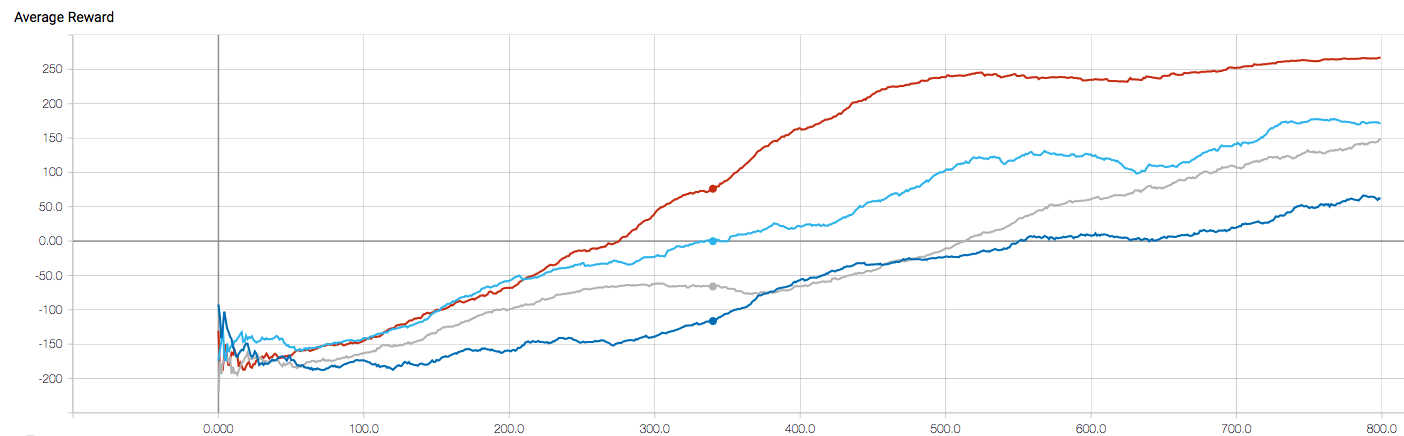
\includegraphics[scale=0.75,width=0.75\columnwidth]{figures/Hyperparameters1.png}%
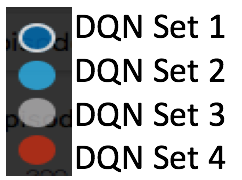
\includegraphics[scale=0.15,width=0.15\columnwidth]{figures/Hyperparameters_legends1.png}%
\caption{ Different Sets of hyperparamerts for DQN Model}%
\label{fig:HyperParameter Table}%
\end{figure}


\label{sec:exp1}
\begin{table}%
%\centering
\begin{tabular}{|l|c|c|c|c|c|}
\hline
Hyper-parameter & Set 1  & Set 2 & Set 3 & Set 4  \\
\hline
gamma & $0.99$ & $0.99$ & $0.99$ & $0.99$ \\
\hline
Epsilon(max,min,decay) & ($1$,$0$,$.998$) &  ($1$,$.01$,$.995$) &  ($1$,$.01$,$.998$) &  ($1$,$.01$,$.998$) \\
\hline
Learning Rate & $0.001$ & $0.0001$ & $0.0001$ & $0.0001$ \\
\hline
DNN layers & [$32$,$32$] &  [$128$,$32$] &  [$128$,$64$] &  [$128$,$64$] \\
\hline
Loss Function & MSE & MSE & MSE & MSE \\
\hline
Batch Size & $32$ & $32$  & $64$  & $64$  \\
\hline
Replay Memory Size & $2^16$ & $2^16$  & $2^16$  & $2^16$  \\
\hline
\end{tabular}
\caption{Different set of hyper-parameters were tried}
\label{tab:Hyper Parameter Set table}
\end{table}
%\vfill}
\subsection{ Error Analysis}
 After doing hyper-parameter tuning, our Agent was able to achieve average score of more than 200 quickly (at 435 episodes). 
However for some episodes after 435 the rewards were not consistently more than 200 for 100 iterations. This is due to the speed 
which is not getting reduced to zero (end state) although Lander is in landing zone.  The lunar lander is trying to bring itself to a zero velocity state and it tries to do so by applying thrust in opposite direction of landing horizontal velocity. In process of doing this, it applies alternate thrust from left and right side but is not able to bring the lander to complete halt to end the episode. Thus reducing the overall rewards and increases the number of frames. We observed that rewards are less than 200 when number of frames reaches the maximum value(1000). The Lunar Lander needs to learn how not to apply alternate left and right thrust to bring itself to a halt, taking no action will be the best action in this state. \\

Also, we observe the variation is more in DQN and Double DQN as compared to Dueling DQN. We got the best performance on Set 4 with Dueling DQN model.

\begin{figure}[!ht]
%\begin{figure}%
%\vspace*{\fill}
\centering
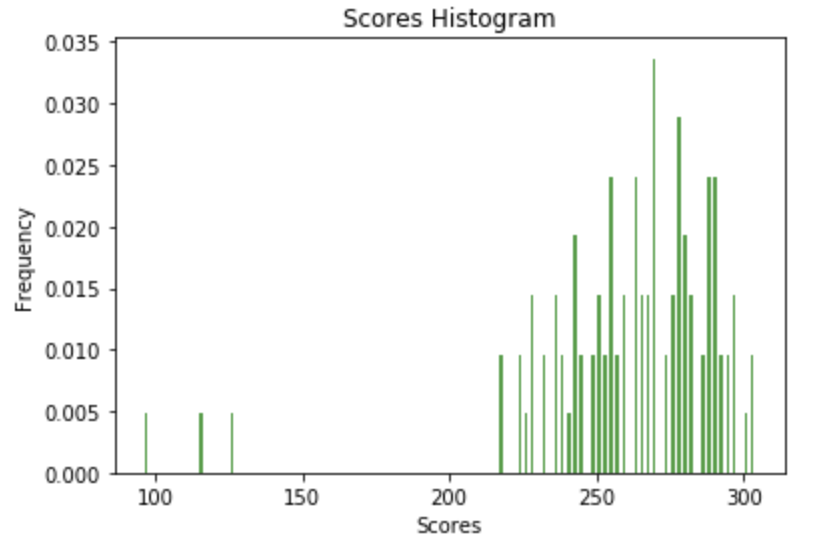
\includegraphics[scale=0.50,width=0.50\columnwidth]{figures/Histogram.png}%
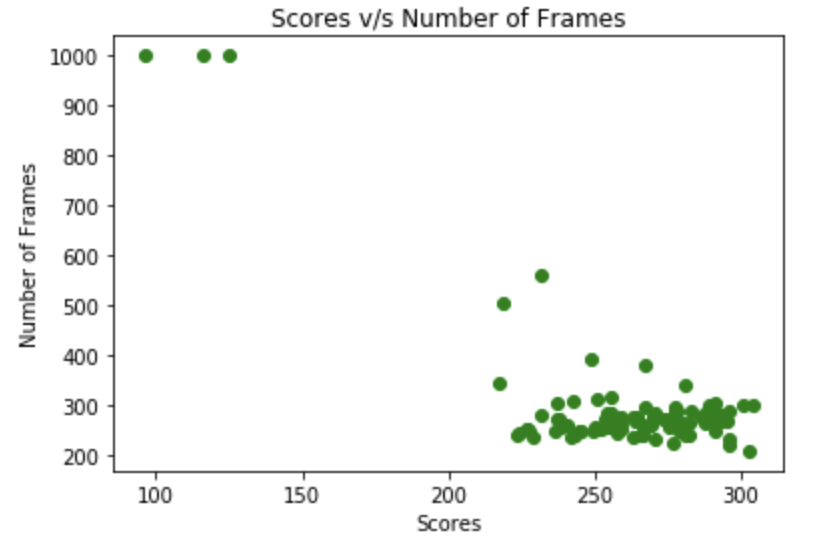
\includegraphics[scale=0.50,width=0.50\columnwidth]{figures/Frames.png}%
\caption{ Error Analysis : Distribution of scores for 100 episodes }%
\label{fig:Error Analysis}%
\end{figure}
%\vfill}

\subsection{ Comparision of DQN Variants}

Comparision of learning for different variants of DQN. 
 
\begin{figure}[!ht]
%\begin{figure}%
%\vspace*{\fill}
\centering
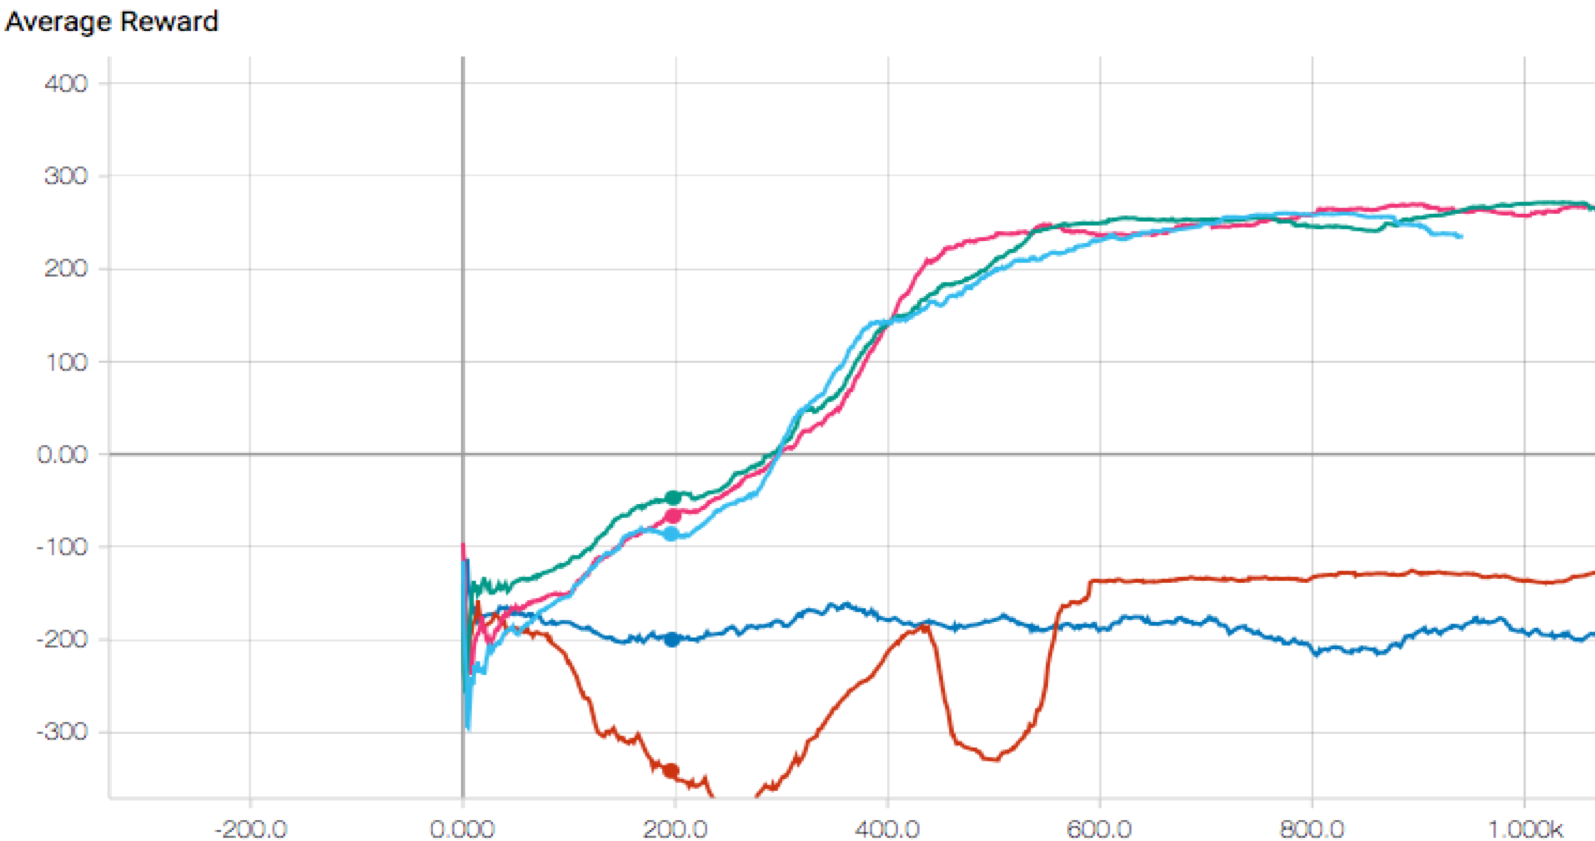
\includegraphics[scale=0.75,width=0.75\columnwidth]{figures/Picture1.png}%
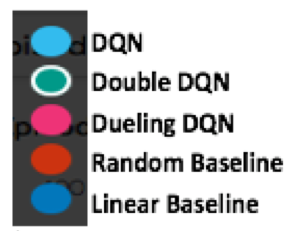
\includegraphics[scale=0.15,width=0.15\columnwidth]{figures/Legend.png}%
\caption{ Rewards for different approaches on tensor board}%
\label{fig:Visualization}%
\end{figure}
%\vfill}

\label{sec:exp}
\begin{table}%
\centering
\begin{tabular}{|l|c|c|}
\hline
Model & Avg. Score  & Number of episodes to reach 200 score  \\
\hline
Baseline & $-200$ & never \\
\hline
Linear Baseline & $-150$ & never \\
\hline
DQN & $123$ & $525$ \\
\hline
Double DQN & $220$ & $500$ \\
\hline
Dueling DQN & $225$ & $435$ \\
\hline
\end{tabular}
\caption{Comparision of Results for different model implementations}
\label{tab:Variants of DQN}
\end{table}


\subsection{ Model Evaluation}

All aforementioned models are evaluated for 100 episodes for a fixed weights. \\  
\begin{figure}[!ht]
%\begin{figure}%
%\vspace*{\fill}
\centering
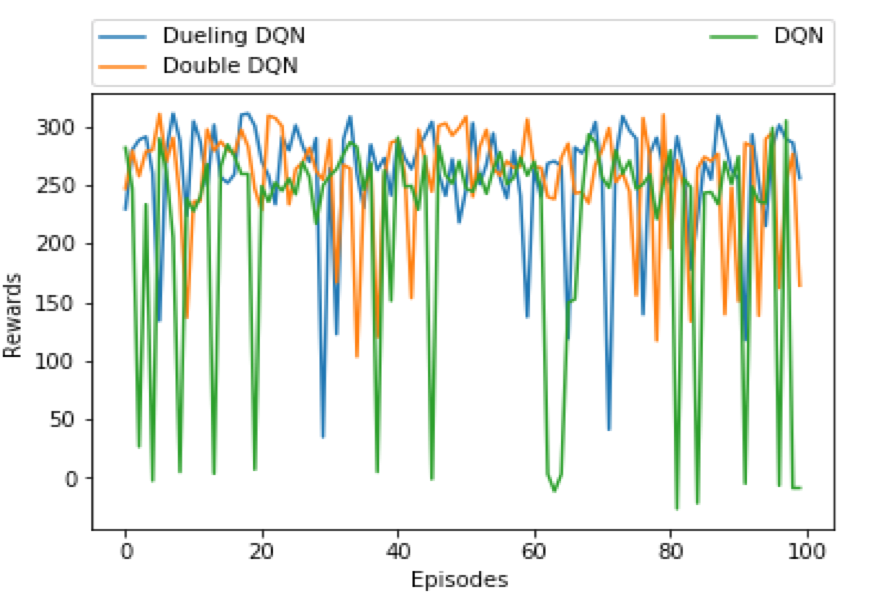
\includegraphics[scale=0.50,width=0.50\columnwidth]{figures/Picture2.png}%
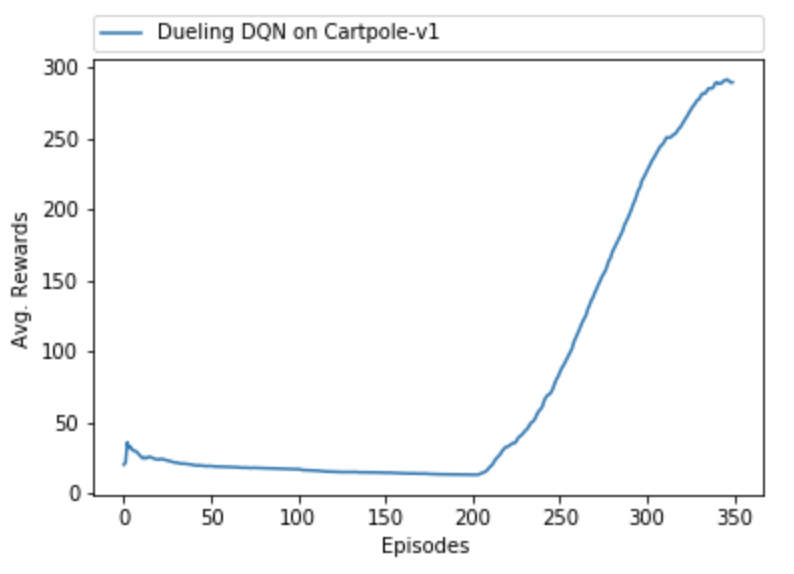
\includegraphics[scale=0.50,width=0.50\columnwidth]{figures/Cartpolev1.png}%
%\caption{ Agent learning CartPole Game}%

\caption{ Evaluating Performance of different DQN Networks and Agent learning CartPole-v1 Game}%
\label{fig:Different DQN Performance}%
\end{figure}
%\vfill}

\subsection{ Agent on other Environments}
We used the Agent to train on "CartPole-v1" game environment and were able to achieve good results. Our AI agent successfully learnt the game and consecutively won it. This proves the generality of the algorithm.

